%package list
\documentclass{article}
\usepackage[top=3cm, bottom=3cm, outer=3cm, inner=3cm]{geometry}
\usepackage{multicol}
\usepackage{graphicx}
\usepackage{url}
%\usepackage{cite}
\usepackage{hyperref}
\usepackage{array}
%\usepackage{multicol}
\newcolumntype{x}[1]{>{\centering\arraybackslash\hspace{0pt}}p{#1}}
\usepackage{natbib}
\usepackage{pdfpages}
\usepackage{multirow}
\usepackage[normalem]{ulem}
\useunder{\uline}{\ul}{}
\usepackage{svg}
\usepackage{xcolor}
\usepackage{listings}
\lstdefinestyle{ascii-tree}{
    literate={├}{|}1 {─}{--}1 {└}{+}1 
  }
\lstset{basicstyle=\ttfamily,
  showstringspaces=false,
  commentstyle=\color{red},
  keywordstyle=\color{blue}
}
%\usepackage{booktabs}
\usepackage{caption}
\usepackage{subcaption}
\usepackage{float}
\usepackage{array}

\newcolumntype{M}[1]{>{\centering\arraybackslash}m{#1}}
\newcolumntype{N}{@{}m{0pt}@{}}


%%%%%%%%%%%%%%%%%%%%%%%%%%%%%%%%%%%%%%%%%%%%%%%%%%%%%%%%%%%%%%%%%%%%%%%%%%%%
%%%%%%%%%%%%%%%%%%%%%%%%%%%%%%%%%%%%%%%%%%%%%%%%%%%%%%%%%%%%%%%%%%%%%%%%%%%%
\newcommand{\itemEmail}{adelgadoal@unsa.edu.pe}
\newcommand{\itemStudent}{Andre David Delgado Allpan}
\newcommand{\itemCourse}{Programación web}
\newcommand{\itemCourseCode}{20231001}
\newcommand{\itemSemester}{III}
\newcommand{\itemUniversity}{Universidad Nacional de San Agustín de Arequipa}
\newcommand{\itemFaculty}{Facultad de Ingeniería de Producción y Servicios}
\newcommand{\itemDepartment}{Departamento Académico de Ingeniería de Sistemas e Informática}
\newcommand{\itemSchool}{Escuela Profesional de Ingeniería de Sistemas}
\newcommand{\itemAcademic}{2023 - A}
\newcommand{\itemInput}{Del 26 Junio 2023}
\newcommand{\itemOutput}{Al 03 Julio 2023}
\newcommand{\itemPracticeNumber}{07}
\newcommand{\itemTheme}{Django Rest Framework}
%%%%%%%%%%%%%%%%%%%%%%%%%%%%%%%%%%%%%%%%%%%%%%%%%%%%%%%%%%%%%%%%%%%%%%%%%%%%
%%%%%%%%%%%%%%%%%%%%%%%%%%%%%%%%%%%%%%%%%%%%%%%%%%%%%%%%%%%%%%%%%%%%%%%%%%%%

\usepackage[english,spanish]{babel}
\usepackage[utf8]{inputenc}
\AtBeginDocument{\selectlanguage{spanish}}
\renewcommand{\figurename}{Figura}
\renewcommand{\refname}{Referencias}
\renewcommand{\tablename}{Tabla} %esto no funciona cuando se usa babel
\AtBeginDocument{%
	\renewcommand\tablename{Tabla}
}

\usepackage{fancyhdr}
\pagestyle{fancy}
\fancyhf{}
\setlength{\headheight}{30pt}
\renewcommand{\headrulewidth}{1pt}
\renewcommand{\footrulewidth}{1pt}
\fancyhead[L]{\raisebox{-0.2\height}{
\includegraphics[width=3cm]{img/logo_episunsa.png}}}
\fancyhead[C]{\fontsize{7}{7}\selectfont	\itemUniversity \\ \itemFaculty \\ \itemDepartment \\ \itemSchool \\ \textbf{\itemCourse}}
\fancyhead[R]{\raisebox{-0.2\height}{
\includegraphics[width=1.2cm]{img/logo_abet}}}
\fancyfoot[L]{Prof. Anibal Sardon }
\fancyfoot[C]{\itemCourse}
\fancyfoot[R]{Página \thepage}

% para el codigo fuente
\usepackage{listings}
\usepackage{color, colortbl}
\definecolor{dkgreen}{rgb}{0,0.6,0}
\definecolor{gray}{rgb}{0.5,0.5,0.5}
\definecolor{mauve}{rgb}{0.58,0,0.82}
\definecolor{codebackground}{rgb}{0.95, 0.95, 0.92}
\definecolor{tablebackground}{rgb}{0.8, 0, 0}

\lstset{frame=tb,
	language=bash,
	aboveskip=3mm,
	belowskip=3mm,
	showstringspaces=false,
	columns=flexible,
	basicstyle={\small\ttfamily},
	numbers=none,
	numberstyle=\tiny\color{gray},
	keywordstyle=\color{blue},
	commentstyle=\color{dkgreen},
	stringstyle=\color{mauve},
	breaklines=true,
	breakatwhitespace=true,
	tabsize=3,
	backgroundcolor= \color{codebackground},
}

\begin{document}
	
	\vspace*{10px}
	
	\begin{center}	
		\fontsize{17}{17} \textbf{ Informe de Laboratorio \itemPracticeNumber}
	\end{center}
	\centerline{\textbf{\Large Tema: \itemTheme}}
	%\vspace*{0.5cm}	

	\begin{flushright}
		\begin{tabular}{|M{2.5cm}|N|}
			\hline 
			\rowcolor{tablebackground}
			\color{white} \textbf{Nota}  \\
			\hline 
			     \\[30pt]
			\hline 			
		\end{tabular}
	\end{flushright}	

	\begin{table}[H]
		\begin{tabular}{|x{4.7cm}|x{4.8cm}|x{4.8cm}|}
			\hline 
			\rowcolor{tablebackground}
			\color{white} \textbf{Estudiante} & \color{white}\textbf{Escuela}  & \color{white}\textbf{Asignatura}   \\
			\hline 
			{\itemStudent \par \itemEmail} & \itemSchool & {\itemCourse \par Semestre: \itemSemester \par Código: \itemCourseCode}     \\
			\hline 			
		\end{tabular}
	\end{table}		
	
	\begin{table}[H]
		\begin{tabular}{|x{4.7cm}|x{4.8cm}|x{4.8cm}|}
			\hline 
			\rowcolor{tablebackground}
			\color{white}\textbf{Laboratorio} & \color{white}\textbf{Tema}  & \color{white}\textbf{Duración}   \\
			\hline 
			\itemPracticeNumber & \itemTheme & 04 horas   \\
			\hline 
		\end{tabular}
	\end{table}
	
	\begin{table}[H]
		\begin{tabular}{|x{4.7cm}|x{4.8cm}|x{4.8cm}|}
			\hline 
			\rowcolor{tablebackground}
			\color{white}\textbf{Semestre académico} & \color{white}\textbf{Fecha de inicio}  & \color{white}\textbf{Fecha de entrega}   \\
			\hline 
			\itemAcademic & \itemInput &  \itemOutput  \\
			\hline 
		\end{tabular}
	\end{table}
	\section{URL de Repositorio Github}
	\begin{itemize}
		
		\item URL para el laboratorio 01 en el Repositorio GitHub.
		\item \url{https://github.com/andre98652/pweb-lab8.git}
	\end{itemize}
	\section{Ejercicio}
	\begin{itemize}
		\item Practique desarrollando el ejerccio de iniciación:
		\item \url{https://www.django-rest-framework.org/tutorial/quickstart/}
		\item Para consumir el web-service puede usar el cliente SOAP UI Community:\url{https://www.soapui.org/downloads/soapui/}
	\end{itemize}
	\section{Tarea}
	\begin{itemize}		
		\item En sus grupos de trabajo correspondientes. Elabore un servicio web que tenga un CRUD con el
uso de este framework.
		\item Create - POST	
		\item Read - GET
		\item Update - PUT
		\item Delete - DELETE
		\item Centrarce en el Core business de su aplicación web. Los más importante y necesario que este disponible a traves de un servicio web.
		\item Ejemplos: \url{https://reqbin.com/, https://www.googleapis.com/youtube/v3/playlistItems}
		\item Muestre la funcionalidad consumiendola desde el cliente Rest de su preferencia.
		
	\end{itemize}
	\subsection{Informe de ejercicio}
	
	\begin{itemize}
		\item Código de app quickstart-serializer.py
	\end{itemize}
	\lstinputlisting[language=Python, 		caption={serializers.py},numbers=left,]{tutorial/tutorial/tutorial/quickstart/serializers.py}
	\begin{itemize}
		\item Código de app quickstart-views.py
	\end{itemize}
	\lstinputlisting[language=Python, 		caption={views.py},numbers=left,]{tutorial/tutorial/tutorial/quickstart/views.py}
	\begin{itemize}
		\item Código del proyecto-settings.py
	\end{itemize}
	\lstinputlisting[language=Python, 		caption={settings.py},numbers=left,]{tutorial/tutorial/tutorial/settings.py}
	\begin{itemize}
		\item Código del proyecto-urls.py
	\end{itemize}
	\lstinputlisting[language=Python, 		caption={urls.py},numbers=left,]{tutorial/tutorial/tutorial/urls.py}
	\begin{itemize}
		\item Captura de la ejecución de ejercicio 
	\end{itemize}
	\begin{figure}[H]
		\centering
		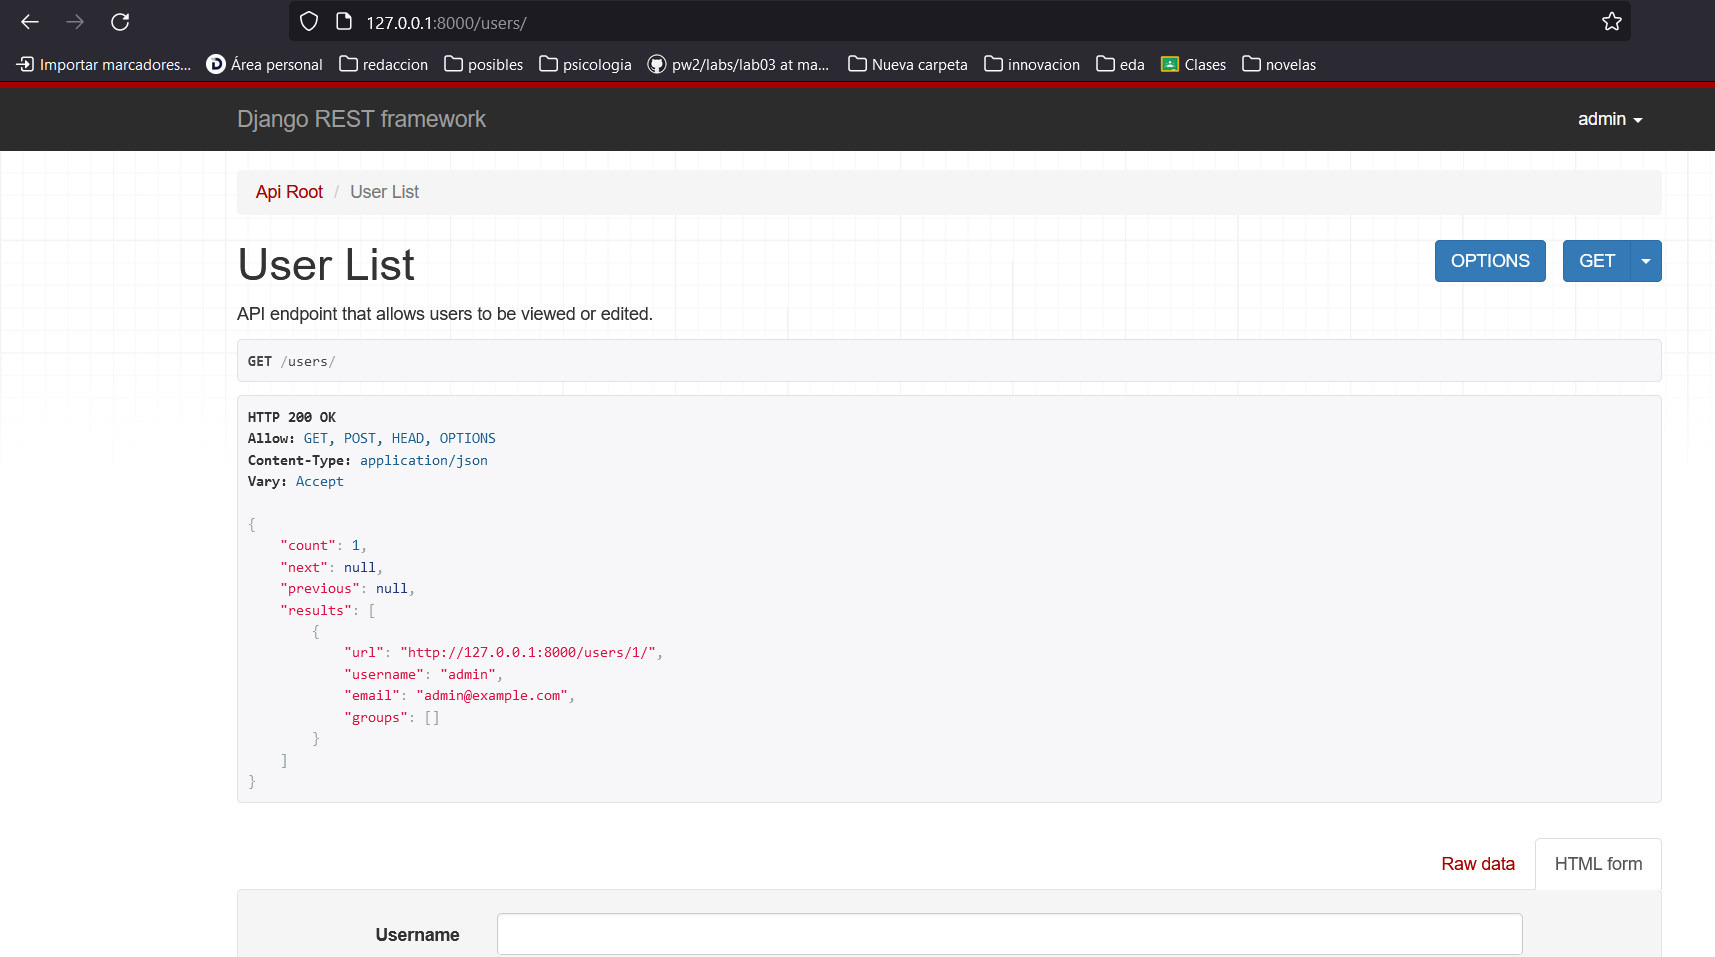
\includegraphics[width=1\textwidth,keepaspectratio]{pruebas/ejercicio.png}
	\end{figure}
	\clearpage
	
	
	
	\section{Informe de tarea}
	\begin{itemize}
		\item Se creo el proyecto api y la aplicacion crud
		\item En la app crud se trabajo con dos modelos autor y libros
		\item Código de app crud-models.py
	\end{itemize}
	\lstinputlisting[language=Python, 		caption={models.py},numbers=left,]{tarea/api/crud/models.py}
	\begin{itemize}
		\item Código de app crud-serializers.py
	\end{itemize}
	\lstinputlisting[language=Python, 		caption={serializers.py},numbers=left,]{tarea/api/crud/serializers.py}
	\begin{itemize}
		\item Código de app crud-views.py, con los metodos requeridos crear, obtener, actulizar y eliminar.
	\end{itemize}
	\lstinputlisting[language=Python, 		caption={views.py},numbers=left,]{tarea/api/crud/views.py}
	\begin{itemize}
		\item Código de app crud-urls.py
	\end{itemize}
	\lstinputlisting[language=Python, 		caption={urls.py},numbers=left,]{tarea/api/crud/urls.py}
	\begin{itemize}
		\item Código del proyecto api-settings.py
	\end{itemize}
	\lstinputlisting[language=Python, 		caption={settings.py},numbers=left,]{tarea/api/api/settings.py}
	\begin{itemize}
		\item Código del proyecto api-urls.py
	\end{itemize}
	\lstinputlisting[language=Python, 		caption={urls.py},numbers=left,]{tarea/api/api/urls.py}
	\begin{itemize}
		\item Captura de la lista de autores por formato json pagina web
	\end{itemize}
	\begin{figure}[H]
		\centering
		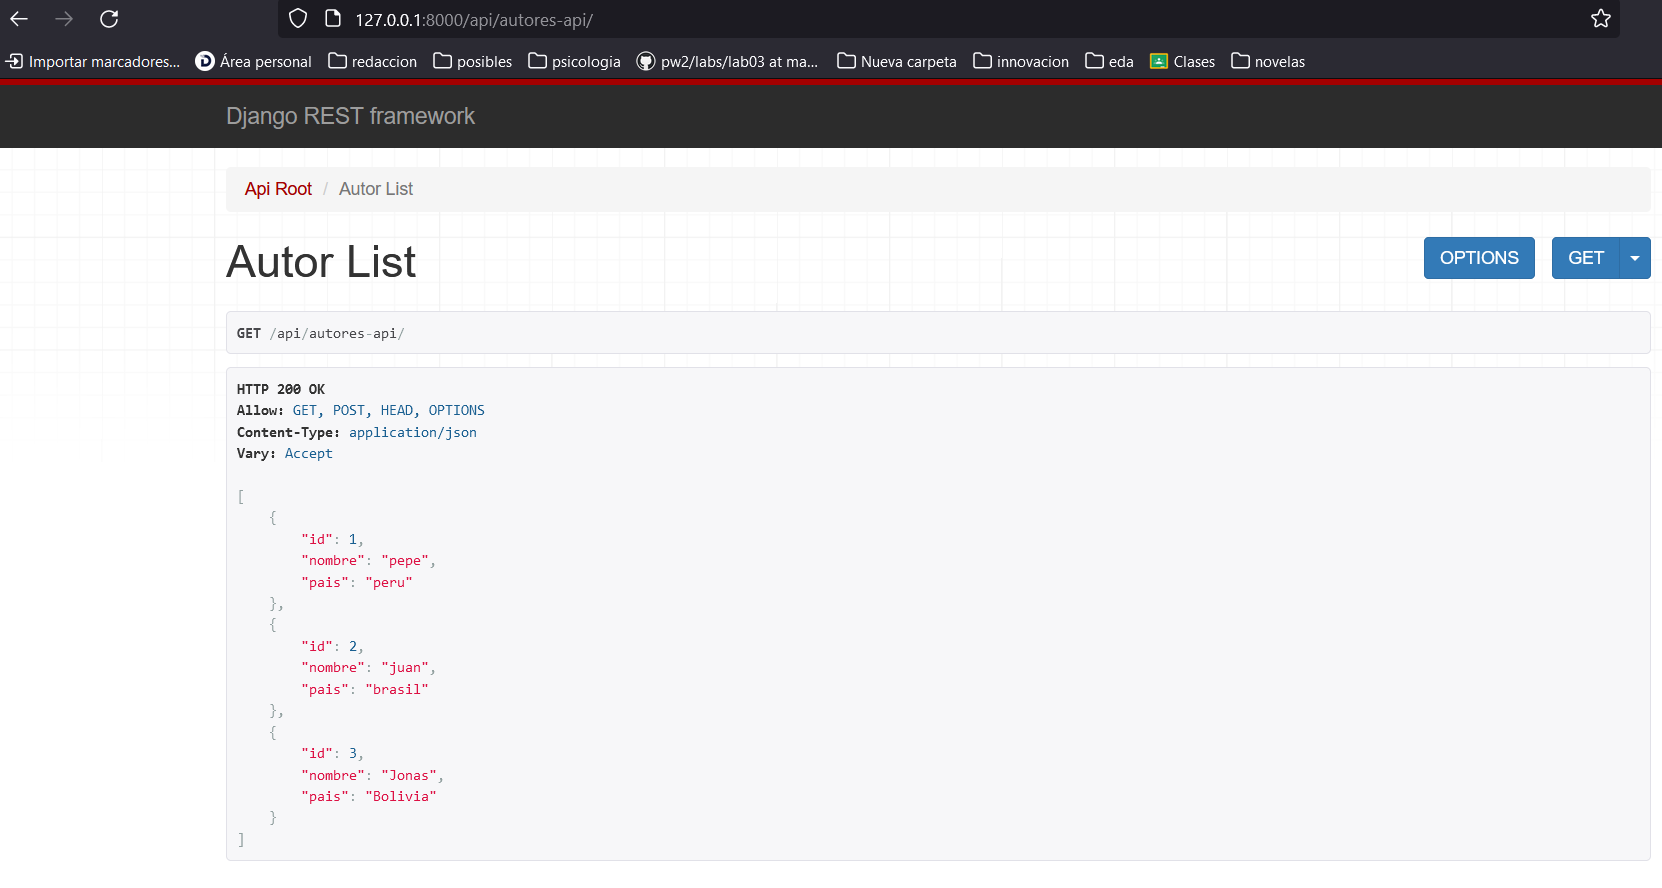
\includegraphics[width=1\textwidth,keepaspectratio]{pruebas/tarea-autores.png}
	\end{figure}
	\clearpage
	\begin{itemize}
		\item Captura de la lista de libros por formato json pagina web
	\end{itemize}
	\begin{figure}[H]
		\centering
		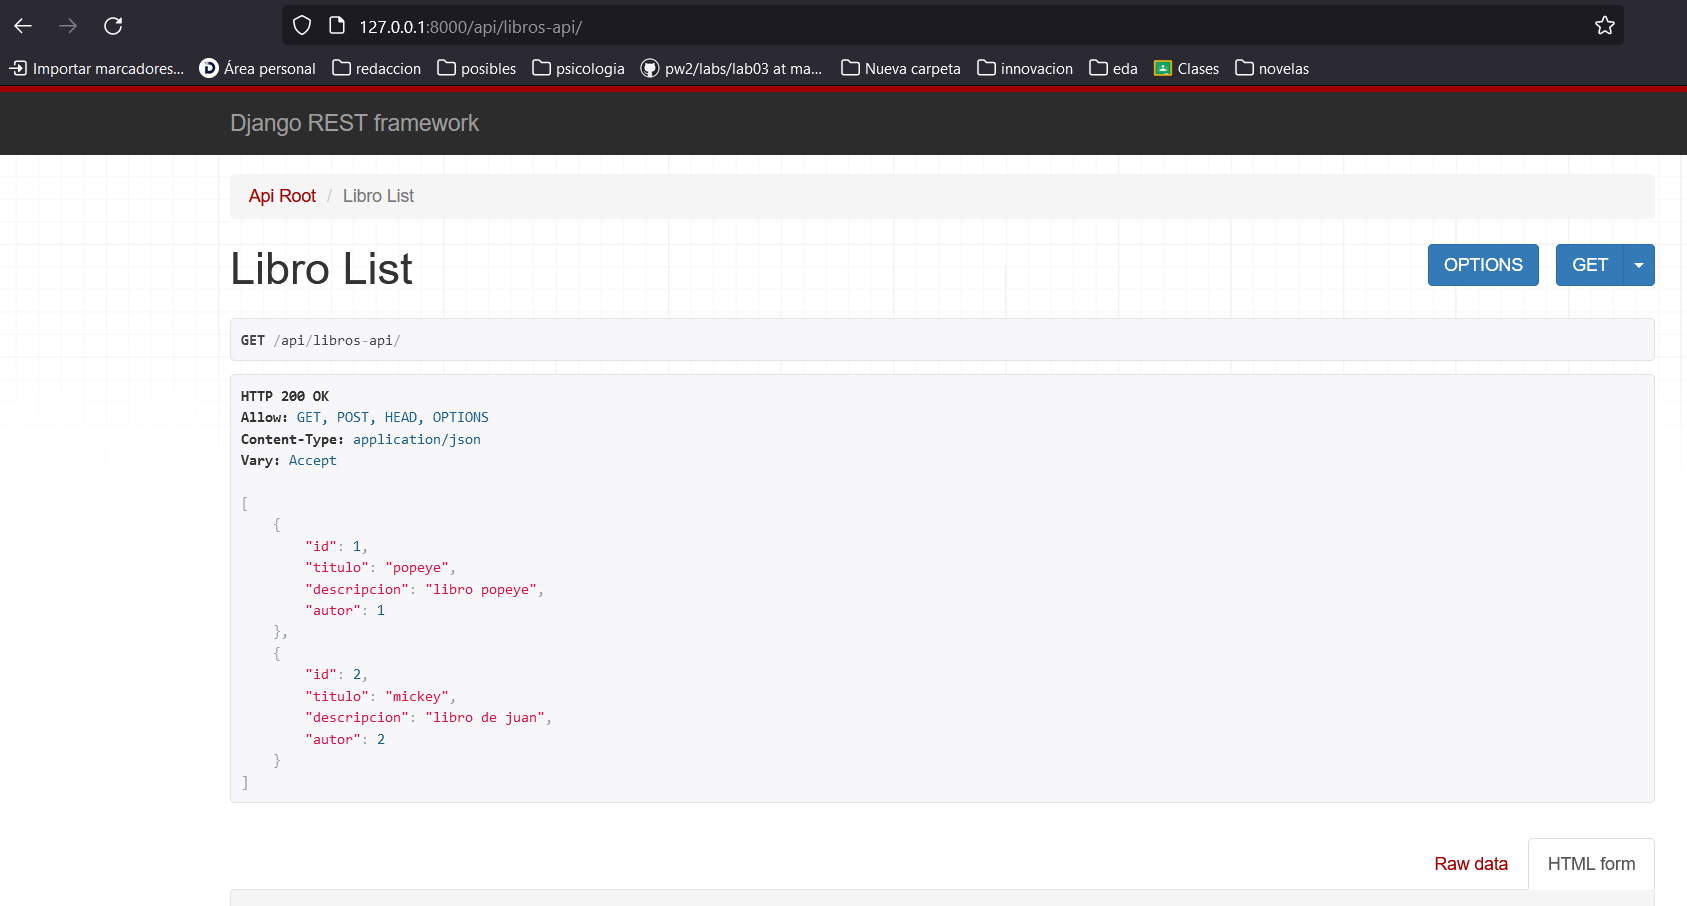
\includegraphics[width=1\textwidth,keepaspectratio]{pruebas/tarea-libros.png}
	\end{figure}
	\clearpage	
	
	
	\section{Consumiendo la API }
	\begin{itemize}
		\item curl para ingresar un autor, METODO POST
	\end{itemize}
	\begin{figure}[H]
		\centering
		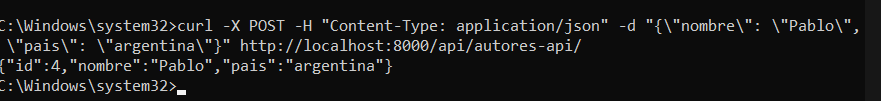
\includegraphics[width=1\textwidth,keepaspectratio]{pruebas/curlIngresarAutor.png}
	\end{figure}
	\begin{figure}[H]
		\centering
		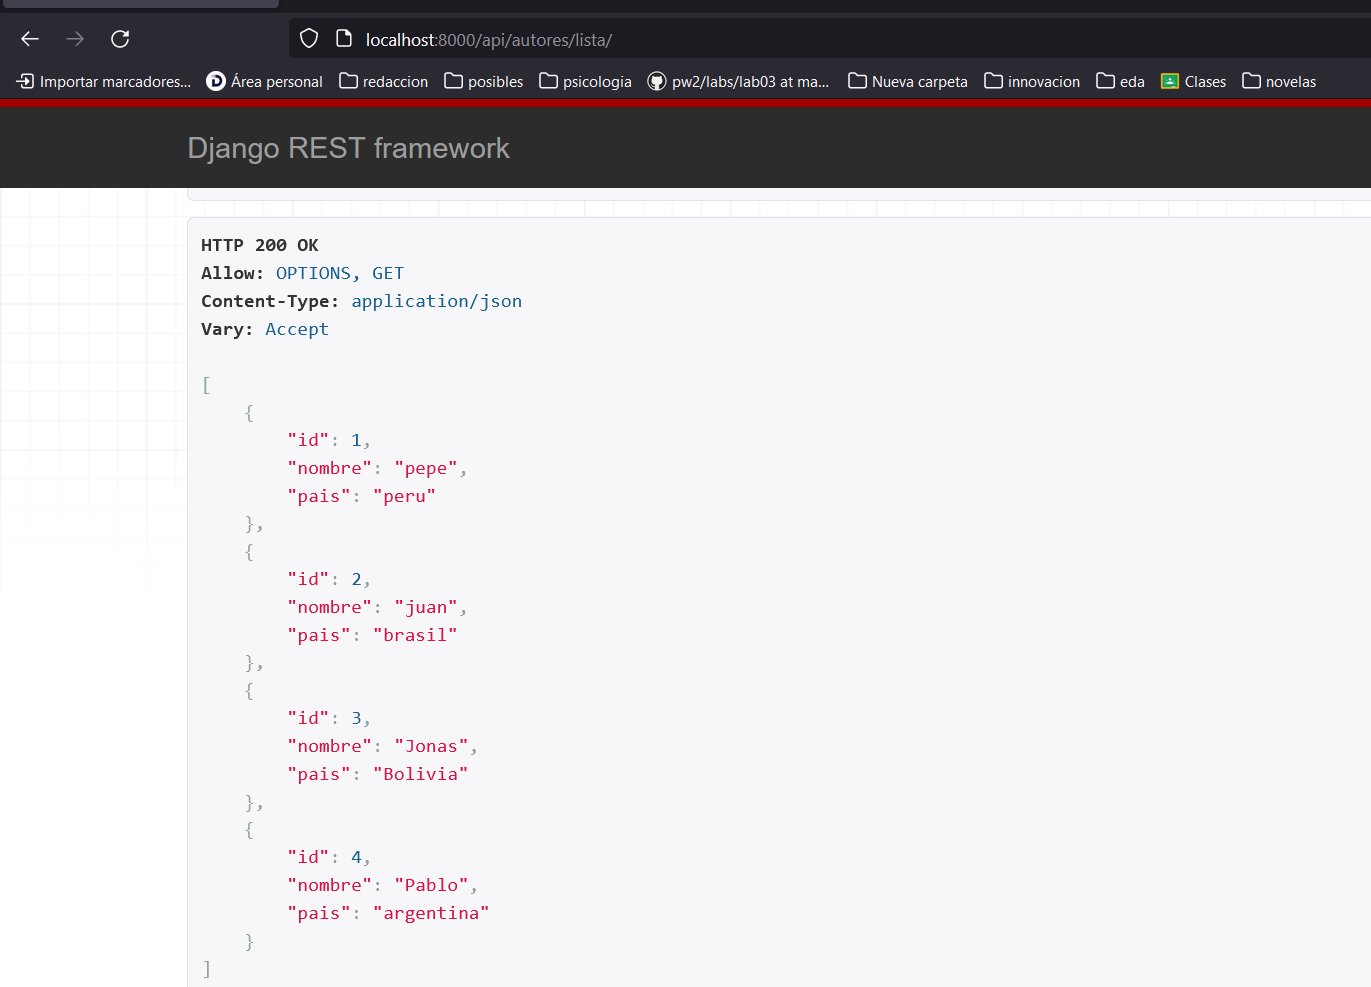
\includegraphics[width=1\textwidth,keepaspectratio]{pruebas/ingresandoAutor.png}
	\end{figure}
	\clearpage
	
	\begin{itemize}
		\item curl para obtener la lista autores, METODO GET
	\end{itemize}
	\begin{figure}[H]
		\centering
		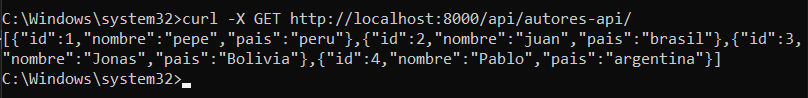
\includegraphics[width=1\textwidth,keepaspectratio]{pruebas/curlObtenerAutores.png}
	\end{figure}
	
	\begin{itemize}
		\item curl para obtener autor por ID, METODO GET
	\end{itemize}
	\begin{figure}[H]
		\centering
		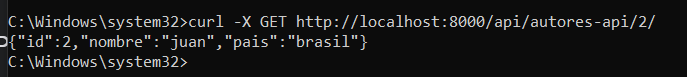
\includegraphics[width=1\textwidth,keepaspectratio]{pruebas/curlObtenerAutorId.png}
	\end{figure}
	
	\begin{itemize}
		\item curl para eliminar autor por ID, METODO DELETE
	\end{itemize}
	\begin{figure}[H]
		\centering
		
\includegraphics[width=1\textwidth,keepaspectratio]{pruebas/curlEliminarAutor.png}
	\end{figure}
	\begin{figure}[H]
		\centering
		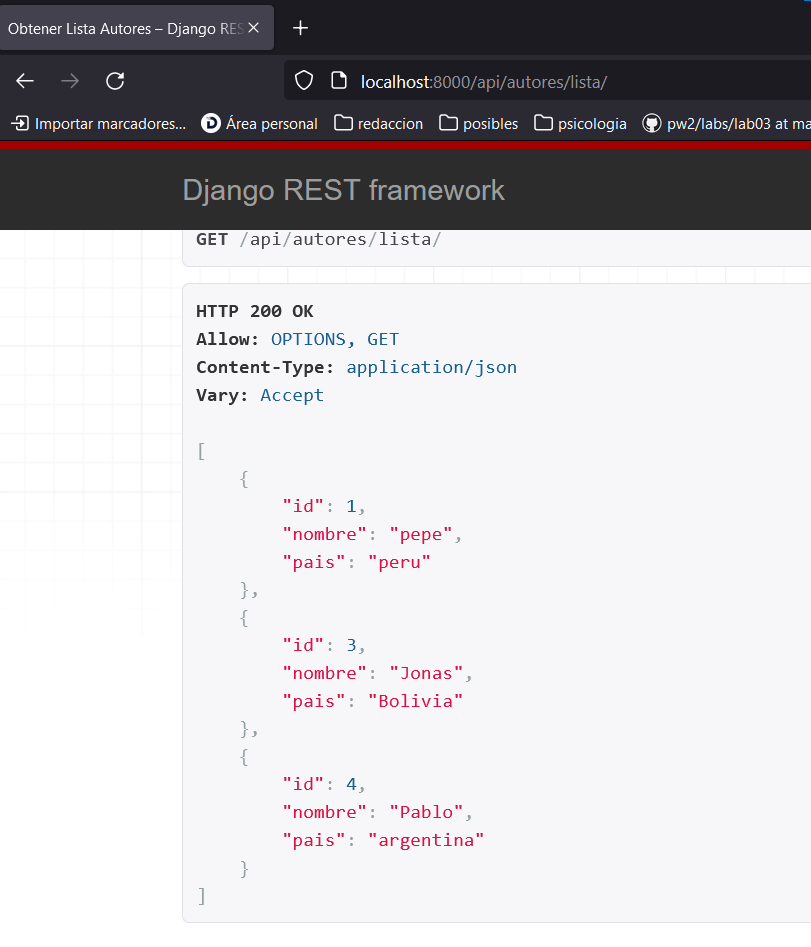
\includegraphics[width=1\textwidth, height=0.8\textwidth,keepaspectratio]{pruebas/tarea-autores-eliminado.png}
	\end{figure}
	
	\begin{itemize}
		\item Al eliminar ese autor se elimina su libro
	\end{itemize}
	\begin{figure}[H]
		\centering
		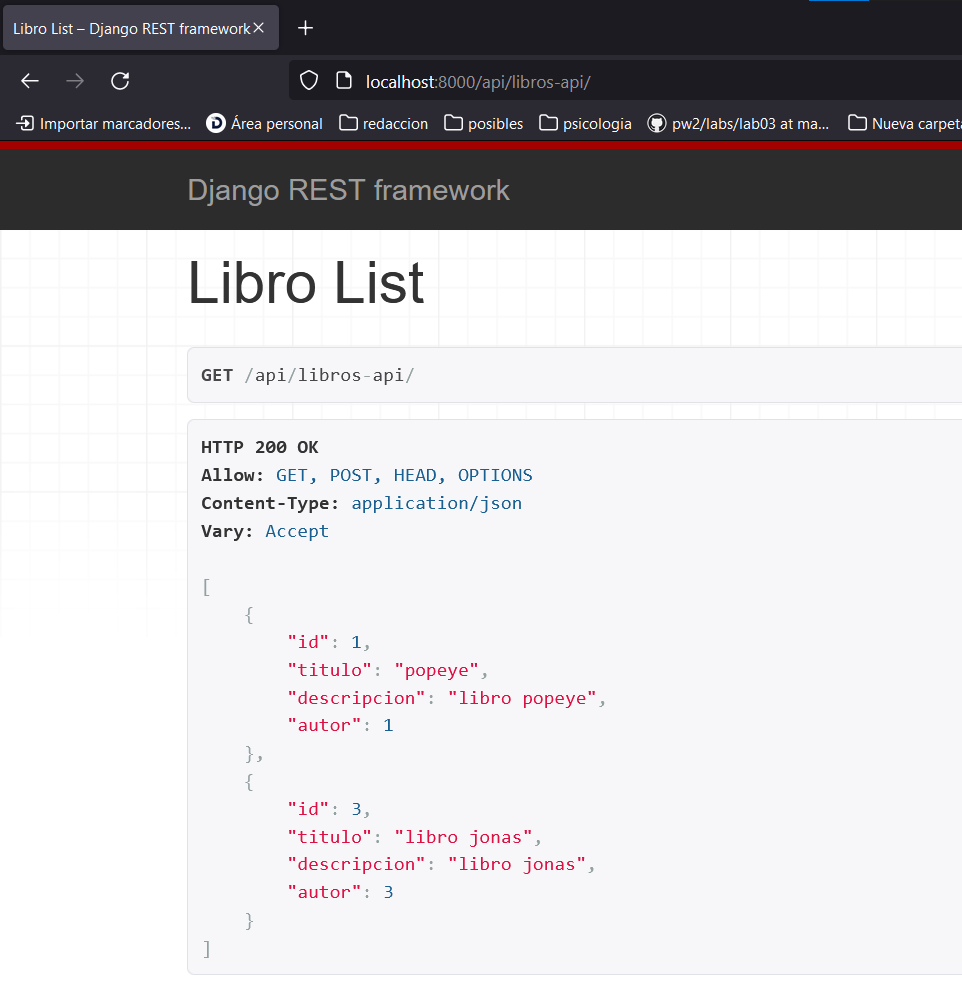
\includegraphics[width=1\textwidth,keepaspectratio]{pruebas/tarea-libros-eliminadoAutor.png}
	\end{figure}
	\clearpage
	
	\begin{itemize}
		\item curl para actualizar autor por ID, METODO PUT
	\end{itemize}
	\begin{figure}[H]
		\centering
		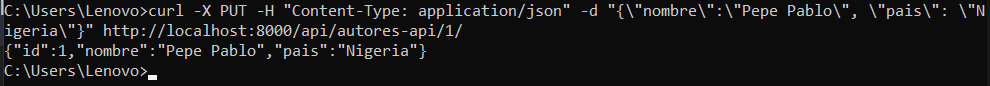
\includegraphics[width=1\textwidth,keepaspectratio]{pruebas/curlActualizarAutor.png}
	\end{figure}
	\begin{figure}[H]
		\centering
		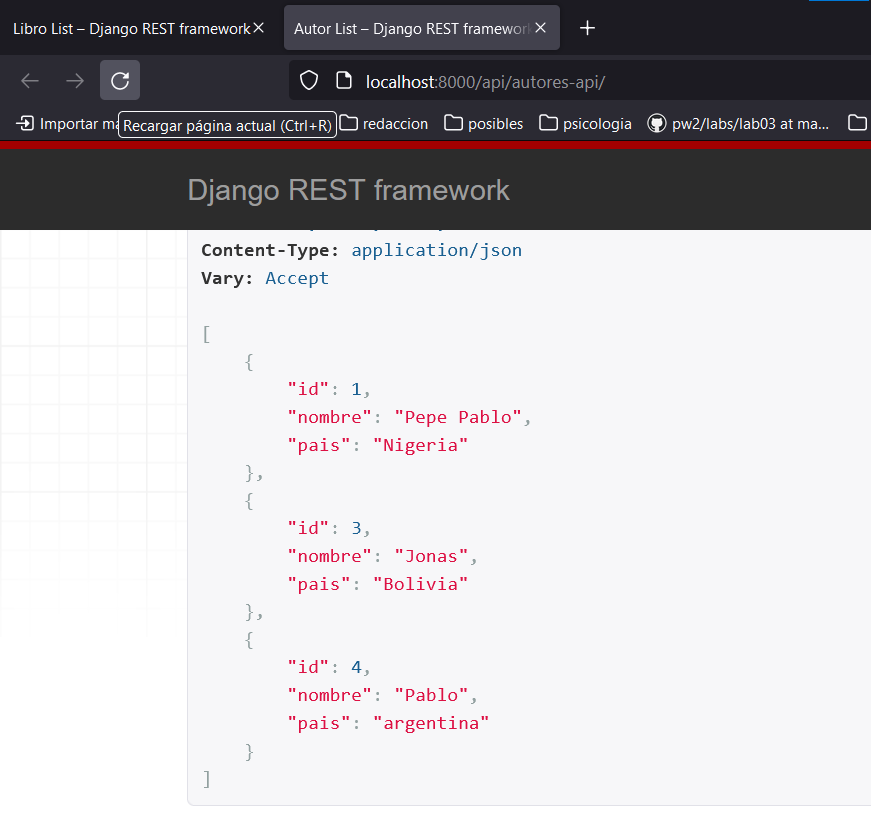
\includegraphics[width=1\textwidth,keepaspectratio]{pruebas/tarea-autores-actualizado2.png}
	\end{figure}
	
	\begin{itemize}
		\item curl para obtener lista de libros, METODO GET
	\end{itemize}
	\begin{figure}[H]
		\centering
		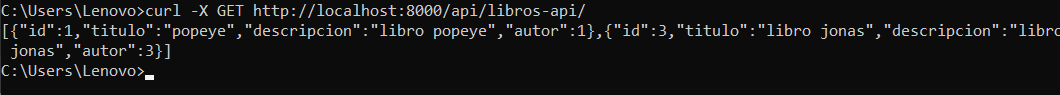
\includegraphics[width=1\textwidth,keepaspectratio]{pruebas/curlObtenerLibro.png}
	\end{figure}
	\clearpage	
	
	\begin{itemize}
		\item curl para ingresar libro, METODO POST
	\end{itemize}
	\begin{figure}[H]
		\centering
		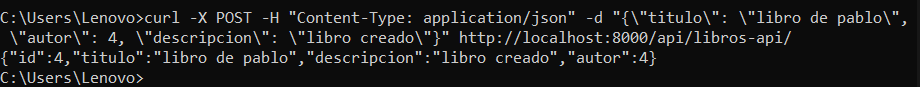
\includegraphics[width=1\textwidth,keepaspectratio]{pruebas/curlIngresarLibro.png}
	\end{figure}
	\begin{figure}[H]
		\centering
		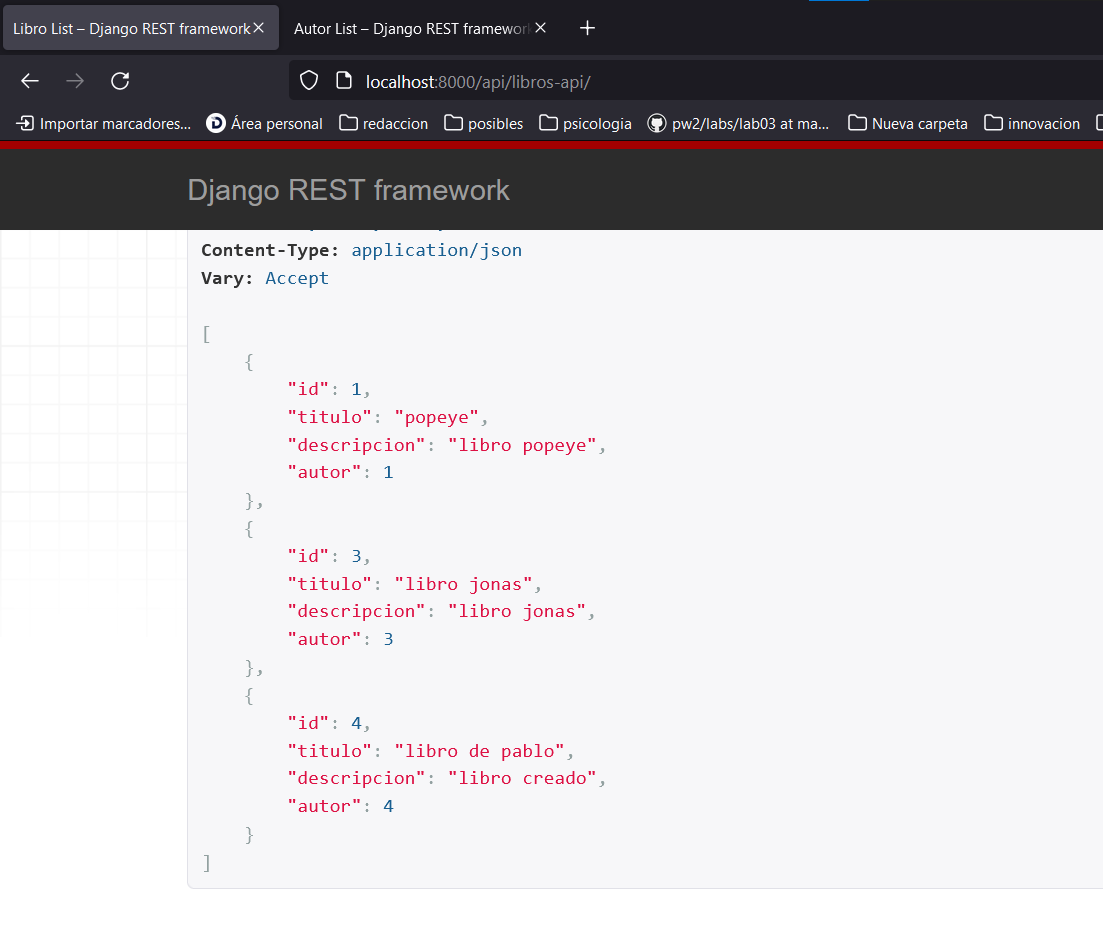
\includegraphics[width=1\textwidth,keepaspectratio]{pruebas/tarea-libro-ingresado.png}
	\end{figure}
	\clearpage
	
	\begin{itemize}
		\item curl para obtener libro por ID, METODO GET
	\end{itemize}
	\begin{figure}[H]
		\centering
		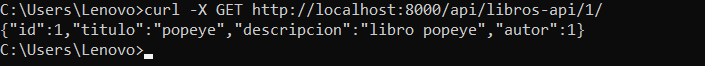
\includegraphics[width=1\textwidth,keepaspectratio]{pruebas/curlObtenerLibroId.png}
	\end{figure}
	
	\begin{itemize}
		\item curl para  actualizar libro por ID, METODO PUT
	\end{itemize}
	\begin{figure}[H]
		\centering
		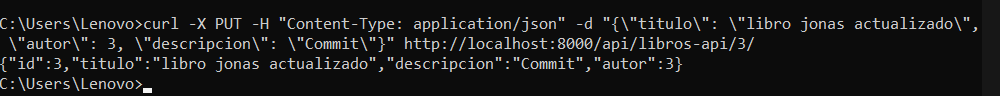
\includegraphics[width=1\textwidth,keepaspectratio]{pruebas/curlActualizarLibro.png}
	\end{figure}
	\begin{figure}[H]
		\centering
		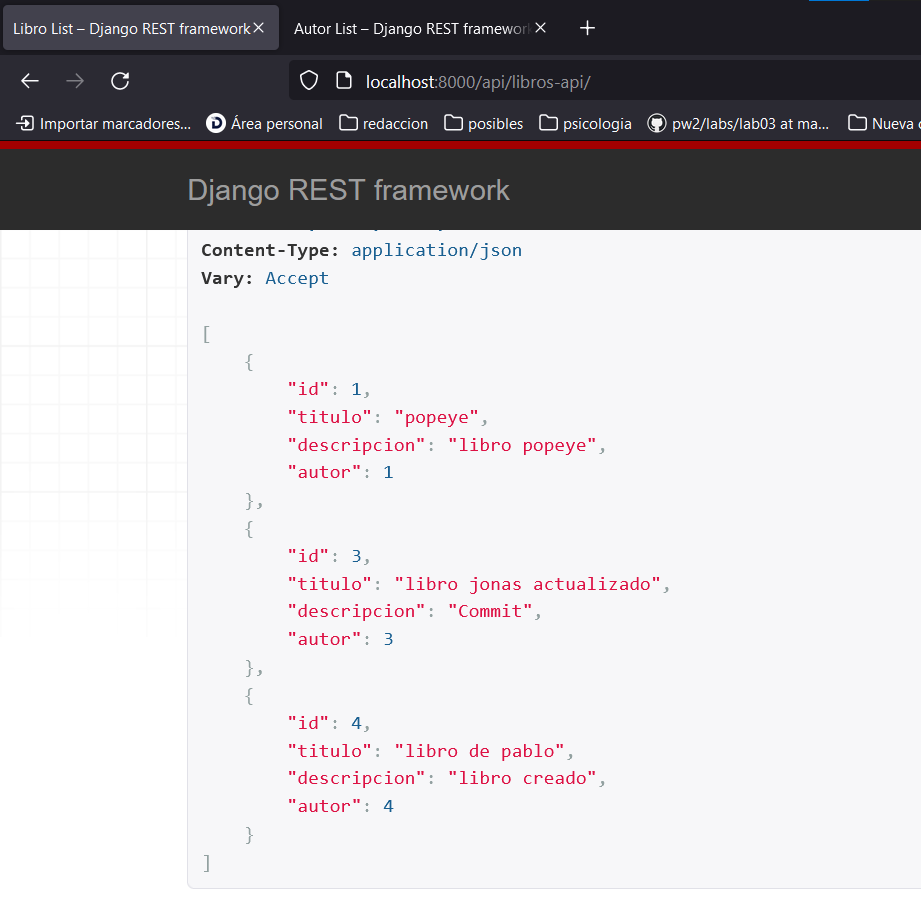
\includegraphics[width=1\textwidth,keepaspectratio]{pruebas/tarea-libro-actualizado.png}
	\end{figure}
	
	\begin{itemize}
		\item curl para eliminar libro por ID, METODO DELETE
	\end{itemize}
	\begin{figure}[H]
		\centering
		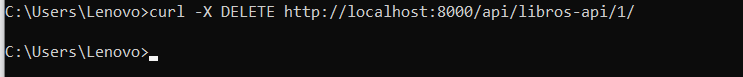
\includegraphics[width=1\textwidth,keepaspectratio]{pruebas/curlEliminarLibro.png}
	\end{figure}
	\begin{figure}[H]
		\centering
		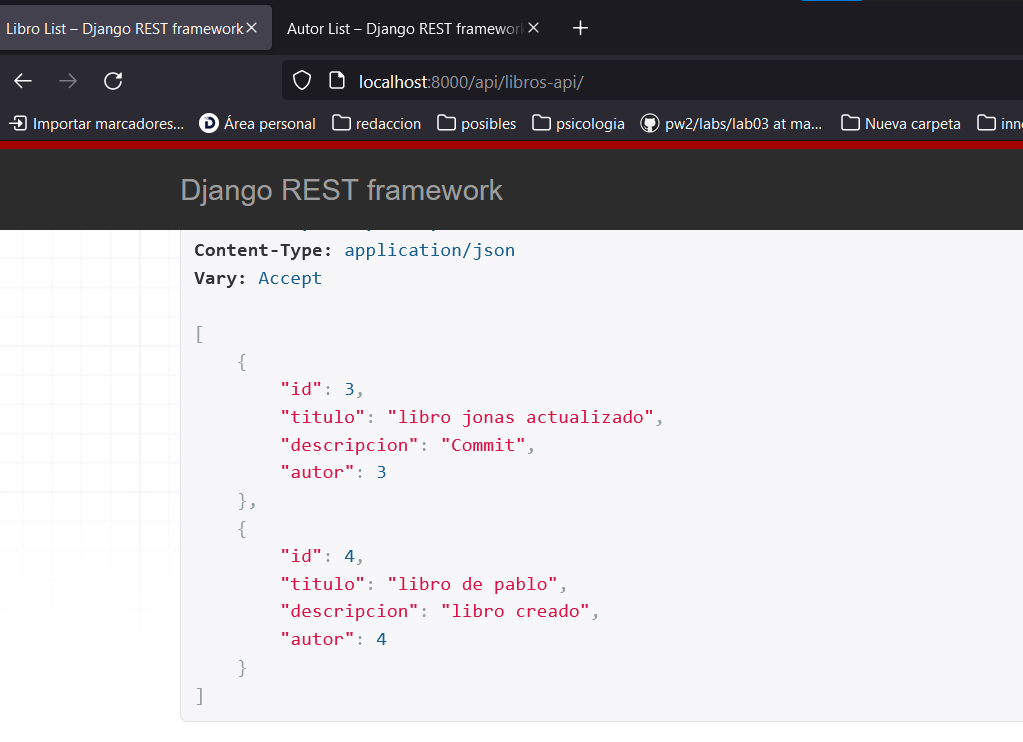
\includegraphics[width=1\textwidth,keepaspectratio]{pruebas/tarea-libro-eliminadoLibro.png}
	\end{figure}
	\section{Cuestionario}
\begin{itemize}
	\item \textbf{¿Cuál fue la mayor dificultad del uso de este framework?} \\
		La mayor dificultad del uso de este framework fue la curva de aprendizaje inicial y la comprensión completa de sus conceptos y funcionamiento. Al ser un framework completo y robusto, Django tiene una amplia gama de características y funcionalidades que pueden resultar abrumadoras al principio.

Además, la configuración inicial del proyecto y la comprensión de la estructura de directorios pueden ser un desafío, especialmente para aquellos que son nuevos en el desarrollo web o en el uso de frameworks.

	
\end{itemize}
	\clearpage
	
	
	\section{\textcolor{red}{Rúbricas}}
	
	\subsection{\textcolor{red}{Entregable Informe}}
	\begin{table}[H]
		\caption{Tipo de Informe}
		\setlength{\tabcolsep}{0.5em} % for the horizontal padding
		{\renewcommand{\arraystretch}{1.5}% for the vertical padding
		\begin{tabular}{|p{3cm}|p{12cm}|}
			\hline
			\multicolumn{2}{|c|}{\textbf{\textcolor{red}{Informe}}}  \\
			\hline 
			\textbf{\textcolor{red}{Latex}} & \textcolor{blue}{El informe está en formato PDF desde Latex,  con un formato limpio (buena presentación) y facil de leer.}   \\ 
			\hline 
			
			
		\end{tabular}
	}
	\end{table}
	
	\clearpage
	
	\subsection{\textcolor{red}{Rúbrica para el contenido del Informe y demostración}}
	\begin{itemize}			
		\item El alumno debe marcar o dejar en blanco en celdas de la columna \textbf{Checklist} si cumplio con el ítem correspondiente.
		\item Si un alumno supera la fecha de entrega,  su calificación será sobre la nota mínima aprobada, siempre y cuando cumpla con todos lo items.
		\item El alumno debe autocalificarse en la columna \textbf{Estudiante} de acuerdo a la siguiente tabla:
	
		\begin{table}[ht]
			\caption{Niveles de desempeño}
			\begin{center}
			\begin{tabular}{ccccc}
    			\hline
    			 & \multicolumn{4}{c}{Nivel}\\
    			\cline{1-5}
    			\textbf{Puntos} & Insatisfactorio 25\%& En Proceso 50\% & Satisfactorio 75\% & Sobresaliente 100\%\\
    			\textbf{2.0}&0.5&1.0&1.5&2.0\\
    			\textbf{4.0}&1.0&2.0&3.0&4.0\\
    		\hline
			\end{tabular}
		\end{center}
	\end{table}	
	
	\end{itemize}
	
	\begin{table}[H]
		\caption{Rúbrica para contenido del Informe y demostración}
		\setlength{\tabcolsep}{0.5em} % for the horizontal padding
		{\renewcommand{\arraystretch}{1.5}% for the vertical padding
		%\begin{center}
		\begin{tabular}{|p{2.7cm}|p{7cm}|x{1.3cm}|p{1.2cm}|p{1.5cm}|p{1.1cm}|}
			\hline
    		\multicolumn{2}{|c|}{Contenido y demostración} & Puntos & Checklist & Estudiante & Profesor\\
			\hline
			\textbf{1. GitHub} & Hay enlace URL activo del directorio para el  laboratorio hacia su repositorio GitHub con código fuente terminado y fácil de revisar. &2 &X &2 & \\ 
			\hline
			\textbf{2. Commits} &  Hay capturas de pantalla de los commits más importantes con sus explicaciones detalladas. (El profesor puede preguntar para refrendar calificación). &4 & & & \\ 
			\hline 
			\textbf{3. Código fuente} &  Hay porciones de código fuente importantes con numeración y explicaciones detalladas de sus funciones. &2 &X &2 & \\ 
			\hline 
			\textbf{4. Ejecución} & Se incluyen ejecuciones/pruebas del código fuente  explicadas gradualmente. &2 &X &2 & \\ 
			\hline			
			\textbf{5. Pregunta} & Se responde con completitud a la pregunta formulada en la tarea.  (El profesor puede preguntar para refrendar calificación).  &2 &X &2 & \\ 
			\hline	
			\textbf{6. Fechas} & Las fechas de modificación del código fuente estan dentro de los plazos de fecha de entrega establecidos. &2 &X &2 & \\ 
			\hline 
			\textbf{7. Ortografía} & El documento no muestra errores ortográficos. &2 &X &2 & \\ 
			\hline 
			\textbf{8. Madurez} & El Informe muestra de manera general una evolución de la madurez del código fuente,  explicaciones puntuales pero precisas y un acabado impecable.   (El profesor puede preguntar para refrendar calificación).  &4 & & & \\ 
			\hline
			\multicolumn{2}{|c|}{\textbf{Total}} &20 & &12 & \\ 
			\hline
		\end{tabular}
		%\end{center}
		%\label{tab:multicol}
		}
	\end{table}
	
\clearpage

\section{Referencias}
\begin{itemize}			
	\item \url{https://www.w3schools.com/java/default.asp}
	\item \url{https://www.geeksforgeeks.org/insertion-sort/}
\end{itemize}	
	
%\clearpage
%\bibliographystyle{apalike}
%\bibliographystyle{IEEEtranN}
%\bibliography{bibliography}
			
\end{document}